\chapter{Spatial Music: Past, Present and Future}
\ref{ch:spat-mus} 

% this chapter is about computer music systems to make spatial music. we will talk about the composer perspective and try to keep the mathematics to a minimum. in later chapters we will focus more on the minutiae of optimizing different systems. here instead we would like to talk about some of the existing software packages in open source computer music languages that can be used to create spatial music. the main focus will be pure data but we can also talk about SuperCollider, Csound, and other tools that might be useful. 

% http://www.iannix.org/ for example. Is an open source tool for graphic scores. Well suited for this chapter. JaroszewiczThesis 

\section{Introduction}

This chapter will be developed with Professor Tom Erbe. In this chapter we will discuss how spatial music has developed over the course of human history. We will talk briefly about some of the composers that broke ground by pioneering compositional techniques and then discuss modern approaches to spatial music by composers such as: Hagan, Lyon, Lopez-Lezcano, Barrett, and many more. 

We will also discuss spatial instruments, which refer to instruments which have considered the manipulation of sound in space as a critical parameter of the instrument design. In contrast to traditional instruments which assume sound radiates outwards from the acoustically activated object, these instruments might not produce any sounds by themselves and instead work in conjunction with computers, which receive data in order to synthesize sound at various real or \textit{phantom} speakers, also known as virtual speakers. 

These instruments are not always entirely electronic - at times we encounter designs in which "traditional" instruments have been extended via the use of sensors to give the performer control over the location of provenance of the sound. Often, computer musicians inextricably tie the development of instruments, or systems, to their compositions in ways that blur the line between: software and score, instrument and composition, or method and material. Some of these \textit{aesthetics} will also be discussed in this chapter. 

Finally, we would like to offer some speculative arguments regarding what the likely direction of spatial music might be in the future. Spatial audio algorithms have been already thoroughly researched for many years. It appears on some level that many of the questions composers sought to ask regarding these systems have already been answered by these various developments. This final section will therefore consider how other technologies might be used in the future towards compositional means based on state-of-the-art research in computer music. 

%These might include advents in Music Information Retrieval (MIR) as well as robotics. 

\section{History of Spatial Music} \label{sec:hist_spat_mus}

% This section will focus on the music from antiquity to the 21st century which uses space as a primary feature of the compositional process. In this chapter, we will trace the development of spatial music from its origins in the 4th century all the way to contemporary works. In future chapters we will seek to speculate how some of the most recent developments in systems design can contribute to this field. It is impossible to address all the works that have been created which fit our parameters, however, we will attempt to present the most important works in the field, as well as some attempts by the author himself to develop works in this space. 

\subsection{Acoustic Music} \label{subsec:acoustic_mus}

Our study of spatial music begins with the very earliest known examples of spatial compositions. \textit{Antiphonal} music is perhaps the oldest of these traditions. The practice of \textit{antiphonal} music, also known as "call and response", can be traced back to Biblical Times, with evidence of its existence as far back as the Roman Catholic Church in the 4th century. In a call and response system, the composer writes melodic lines using tension and resolution with independent choral group assigned different parts of the melody. The composer might create tension by using a dissonant note as the final note of the "calling" phrase. A different group, located in a different location of the stage, would resolve the melodic phrase, usually ending in the tonic of the scale and while the harmony resolves using some traditional cadence\footnote{Like a IV-I, plagal cadence, or a V-I, perfect cadence.}. 

Many of these early works are hard to replicate today due to the lack of documentation. In the 16th century, however, printed works in spatial music would surface. Some of these initial innovative pieces were written by the Flemish composer Adrian Willaert\footnote{Netherlandish composer of the Renaissance.}, for example, whom exploited the \textit{Basilica de San Marco's\footnote{The cathedral church of the Roman Catholic Archdiocese of Venice, northern Italy.}} two organs in antiphonal compositions featuring two separate choirs and multiple instrumental groups \cite{arnold1959significance}. The technique \textit{cori spezzati}, or separated choirs, was re-introduced in his 1550's piece titled \textit{Vespers}, which itself featured multi-part arrangements and echo effects. Willaert's pupil, Andrea Gabrieli, an Italian composer of the late renaissance, would later continue his teacher's work, cementing spatial music as a hallmark of the Venetian musical practice. 

\begin{figure}[ht!]%force figure here, top, strict
\centering
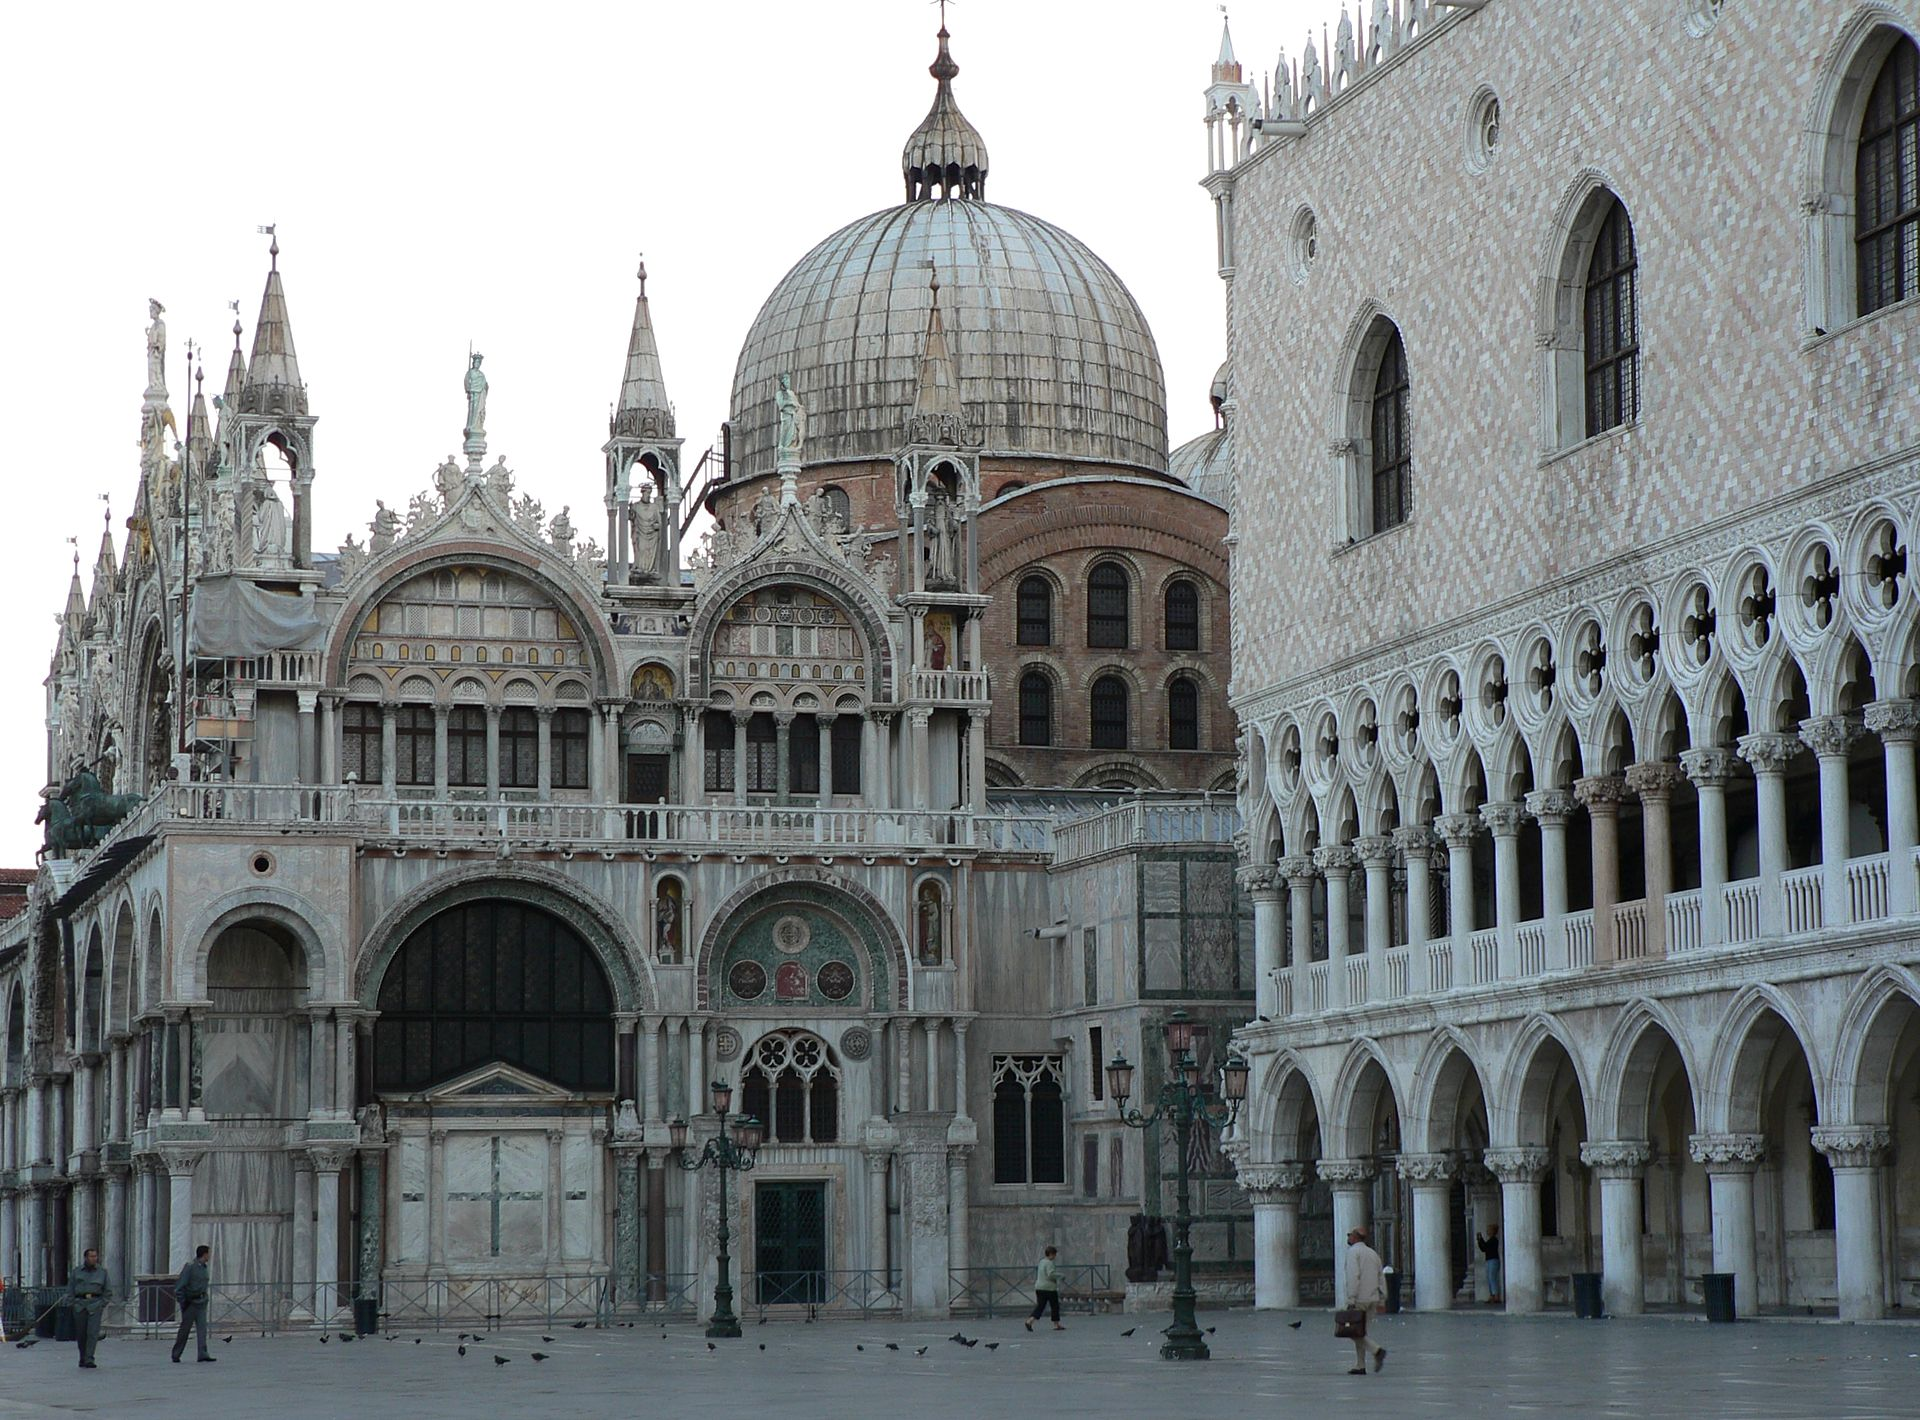
\includegraphics[width=0.7\textwidth]{img/basilica-san-marcos.JPG} 
%\captionsetup{justification=centering}
\caption{Basilica de San Marco - wikimedia commons}
\end{figure}

As a result of Willaert's work the practice of spatial music quickly spread to other parts of Europe where it was quickly adopted by composers such as Thomas Tallis in England. \textit{Spem in alium}, one of Tallis's most famous pieces, was composed for Queen Elizabeth upon her 40th birthday, in 1573, and featured 40 vocal parts arranged in eight 5-voice choirs. The high point of spatial music during the baroque era might however be Orazio Benevoli's\footnote{Franco-Italian composer born in Rome (19 April 1605 – 17 June 1672).} \textit{Festival Mass}, written in 1628 for the \textit{Salzburg Cathedral} which called for 16 vocal parts, 34 instrumental parts, two organs, and a basso continuo\footnote{Figured bass where the most common combination is harpsichord and cello for chord and bass-line respectively.} \cite{zvonar1999history}.

Following the baroque era, interest in spatial music subsided until the beginning of the Romantic period. A key distinction of this era is the use of spatial music for theatrical effect. The romantic period is often characterized by the rise and popularity of operas by composers such as: Hector Berlioz, a French Romantic composer and conductor (11 December 1803 – 8 March 1869) who wrote \textit{Requiem} in 1837, and Gustav Mahler, an Austro-Bohemian Romantic composer (7 July 1860 – 18 May 1911)\footnote{Considered one of the leading conductors of his generation.} who wrote \textit{Symphony No.2} in 1895 \cite{einstein1948music}. These composers not only spaced instruments for their performances but also choreographed the entrance and exiting of musicians as they played, creating some iconic musical moments.

In the 20th century, experimentalists such as Charles Ives, American modernist composer (October 20, 1874 – May 19, 1954), and Luigi Russolo, Italian Futurist composer and the author of the manifesto \textit{The Art of Noises} (30 April 1885 – 6 February 1947), inspired by the tumultuousness of industrial life, refined the art of musical collage using spatial sound \cite{jones199120th}. Ives's 1908 \textit{The Unanswered Question} called for offstage strings. Charles was inspired by his father George, a Civil War bandmaster, and music teacher, who had himself experimented with spatial music in his days. 

Henry Brant\footnote{Canadian-born American composer whom composed numerous orchestral spatial works (September 15, 1913 – April 26, 2008).}, inspired by Ives's music, would go on to create \textit{Antiphony I} (1953) which called for five spatially separated orchestras, and, \textit{Voyage Four} (1963) which called for three conductors to direct: percussion and brass on stage, violins on one balcony, violas and celli on another, basses on the floor level at rear, woodwinds at a rear balcony, and several performers in the audience \cite{zvonar1999history}. Brant's \textit{Windjammer} (1969), likely inspired by the opera composers of the baroque times, featured a static horn soloist and several wind players that moved along prescribed routes as they performed, in a choreographed manner. 

\cite{harley1997american} provides a rich analysis of four of Brant's most important works in the field of spatial music. Brant emphasized the need for differing timbres to be represented in his music, since he believed the heterogeneity would aid in the clarity of the musical representation. Indeed, if multiple instruments of the same family were spatially distributed, it would be difficult to differentiate melodic phrases, especially if these were all playing in the same register. 

Brant summarized his main observations with regards to spatial composition in a 1967 articles paraphrased as following: 

\begin{enumerate}
    \item \textit{Spatial separation clarifies texture}: when multiple musicians play different musical phrases in the same octave range, separating them spatially helps give clarity to each stream. 
    \item \textit{Separate groups are difficult to coordinate}: exact rhythms might be difficult to accomplish due to the distance it takes for sounds to arrive from one playing position to the next. 
    \item \textit{Spatial separation is equivalent to range separation}: it is possible to enhance the texture of a melodic phrase simply my separating musicians playing the same material.  
    \item \textit{Spatial arrangements must allow flexibility}: the specific architectural demands of the works cannot always be met, alternatives should be provided whenever possible.
\end{enumerate}

Brant is perhaps one of the mos prolific composers of acoustic works with a repertoire of 67 spatial pieces. Brant also wrote extensively on the subject of spatial music and experimented at length with form, rhythm and perceptual experience. In contrast to other composers of his era, Brant's music dealt exclusively with acoustic means, which he creatively articulated to provide depth, envelopment and movement.  

\todo[inline]{Still feel like I should say a bit more about Brant. Might add more later.}

\subsection{Electro-acoustic Music} \label{subsec:elec_acoustic_mus}

Along a parallel branch of history there exist a number of musical experiments conducted in the 20th century by avant-garde musicians and composers typically categorized as \textit{electro-acoustical}. This label is used to separate them from traditional composers who avoided electronics or seldom exploited electronics in their compositions. The composers of this space and time were all activated by the development of sound recording, radio and telephony, and used them purposefully in their works. With the possibility of sound as a medium displaced from its source, dozens of new forms of music were created, this section will describe some. 

The birth of recorded sound brought with it an era of technological music development as composers and engineers sought to keep audiences attending live events - if only to see what strange machines were creating the sounds they could hear on their recordings at home. Thaddeus Cahill's \textit{Telharmonium} (1900-1906) is considered the first electrical musical instrument of its kind \cite{bode1984history}. Also known as the Dynamophone, this electrical organ was used to deliver music to homes on a subscription basis via a telephone line. We should note here that the element of space is present in an example such as this one, in a different semantic context, given the distance created between performer and audience. 

% \begin{figure}[ht!]%force figure here, top, strict
% \centering
% 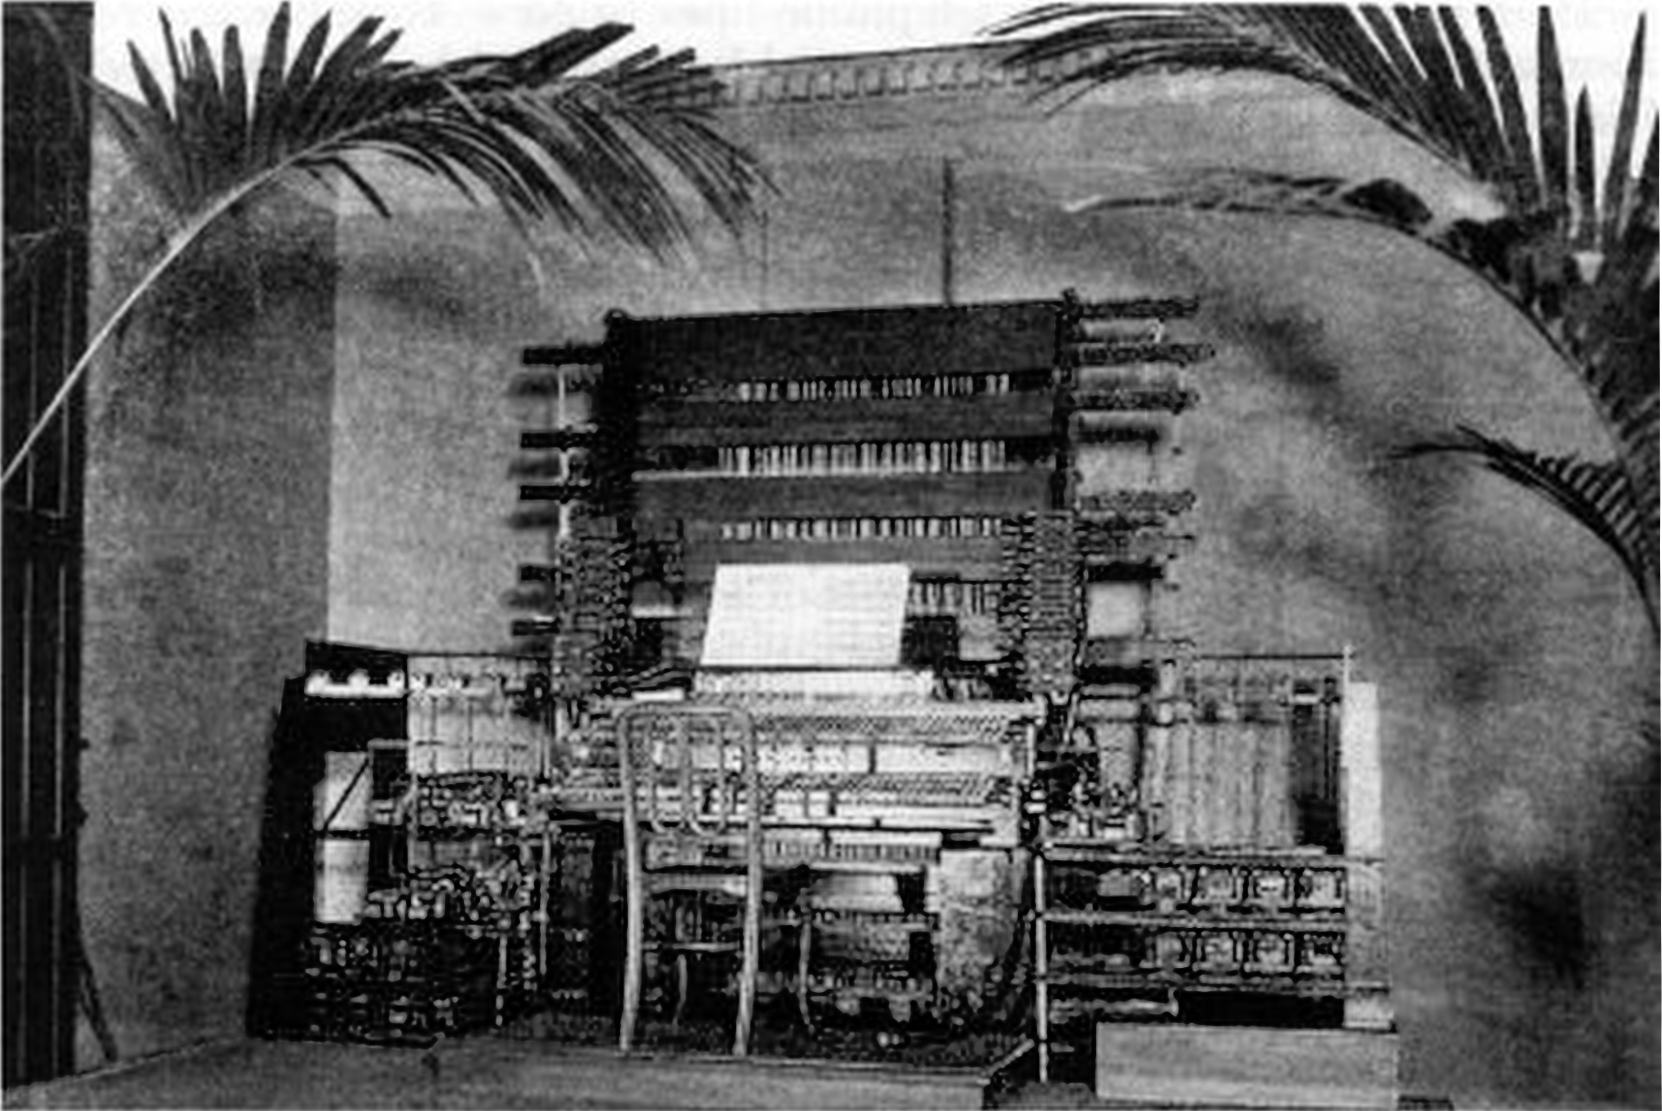
\includegraphics[width=0.8\textwidth]{img/telharmonium.jpg} 
% %\captionsetup{justification=centering}
% \caption{Telharmonium Press - wikimedia commons}
% \end{figure}

Later, in 1923, Leon Theremin would introduce a new instrument to the public. The theremin, named after its inventor, used two antennae to control the pitch and volume of a synthesizer. The user must position their hands in space to control the instrument and produce the desired sound. Theremin later formed ensembles in which multiple theremin were used in one of the first public displays of multi-channel loudspeaker music ever. The theremin is another particularly provoking example as it illustrates not only how space can be used for acoustic effect, but ergonomically speaking, it shows how an instrument can use space to facilitate its playing. Neither of these two instruments, however, exploit psycho-acoustic principles, the development of such instrument would come much later as we will see.  %spatial instrument

\begin{figure}[h!]%force figure here, strict
\centering
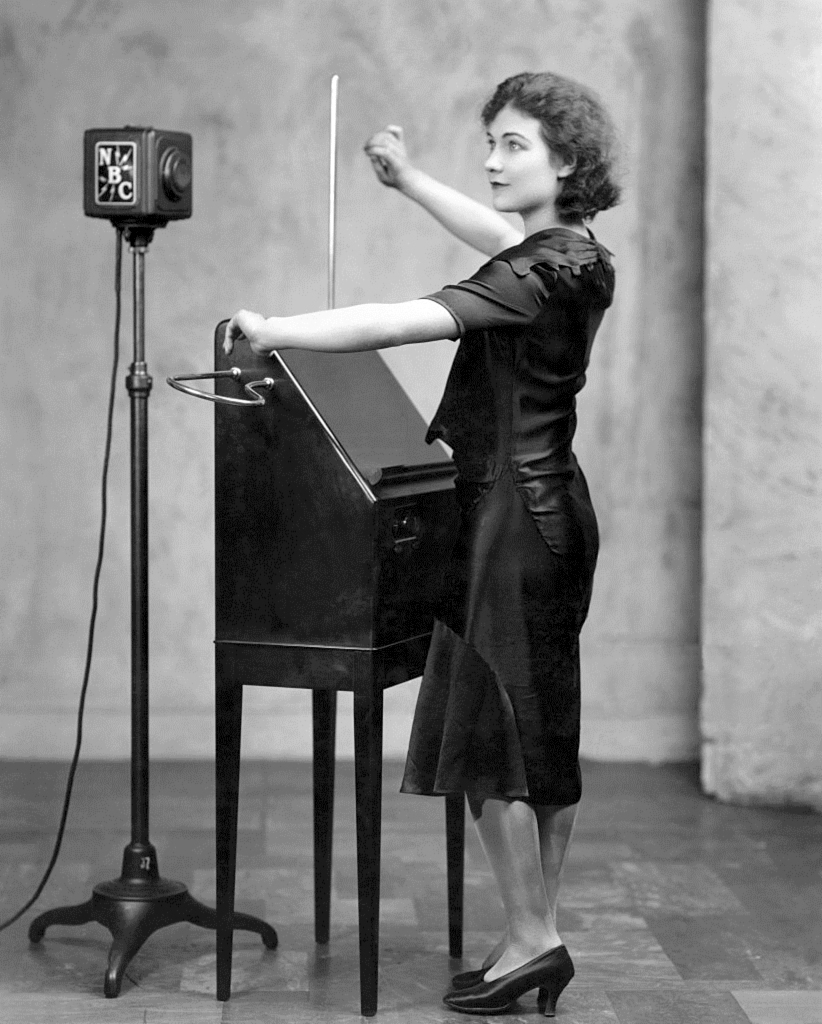
\includegraphics[width=0.5\textwidth]{img/theremin.jpg} 
%\captionsetup{justification=centering}
\caption{Alexandra Stepanoff\protect\footnotemark playing the theremin on NBC Radio, 1930 - wikimedia commons}
\end{figure}

\footnotetext{Alexandra Stepanoff was one of Léon Théremin’s first theremin students in the United States. Formerly a concert singer, around the late twenties, she moved from Russia to New York, where, thanks to the local Russian community, she met Léon Théremin.\cite{2020_stepanoff}}

The 20th century also saw the rise of phonographs\footnote{Colloquially known as record players.} as musical instruments. Paul Hindemith\footnote{Prolific German composer (16 November 1895 – 28 December 1963).} began this practice in the 1920's and 30's nearly 80 years before DJing practices became popular \cite{manning2013electronic}. John Cage\footnote{American avant-garde composer (September 5, 1912 – August 12, 1992).} also adopted the use of phonographs compositionally in \textit{Imaginary Landscape No. 1} (1939) which used multiple turntables and test tones, and in \textit{Imaginary Landscape No. 4} (1951) where he used 12 radios, 24 performers and a conductor. In addition to exploring the use of phonographs as instruments, Cage also exploited radio broadcast and tape in his creative practice.  

% \begin{figure}[ht!]%force figure here, top, strict
% \centering
% 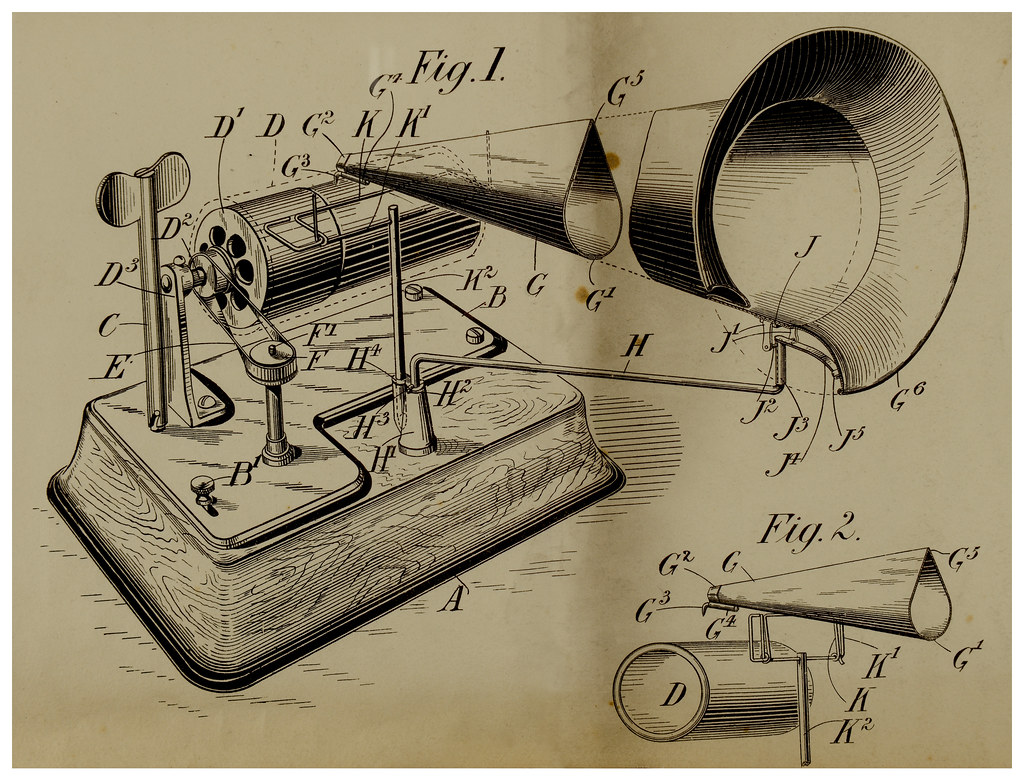
\includegraphics[width=0.5\textwidth]{img/phono.jpg} 
% %\captionsetup{justification=centering}
% \caption{Phonograph - \cite{cc}}
% \end{figure}

By separating the original performer from the playback these composers were playing not just with space, but also time. Cage, along with a group of experimental composers called "Project for Music for Magnetic Tape", would go on to write four pieces for tape \cite{cage1961experimental} during the 50s. The most famous piece that emerged from the group was likely \textit{William's Mix}\footnote{\href{http://tre.ucsd.edu/wordpress/?p=644}{Tom Erbe created a Pd version of William's Mix. (access: Jan 7, 2021)} } (1952) which called for 8 tape machines each played back from its own speaker and hundreds of sounds carefully spliced together. This was one of Cage's first use of chance in musical composition. The project also resulted in works by Earle Brown\footnote{American composer who pioneered the use of graphic scores (December 26, 1926 – July 2, 2002).} (\textit{Octet}) and Morton Feldman\footnote{American composer perhaps best known for his extended works which could last up to six hours (January 12, 1926 – September 3, 1987).} (\textit{Intersection}), both using 8 tape players and speakers. 

\begin{figure}[ht!]%force figure here, top, strict
\centering
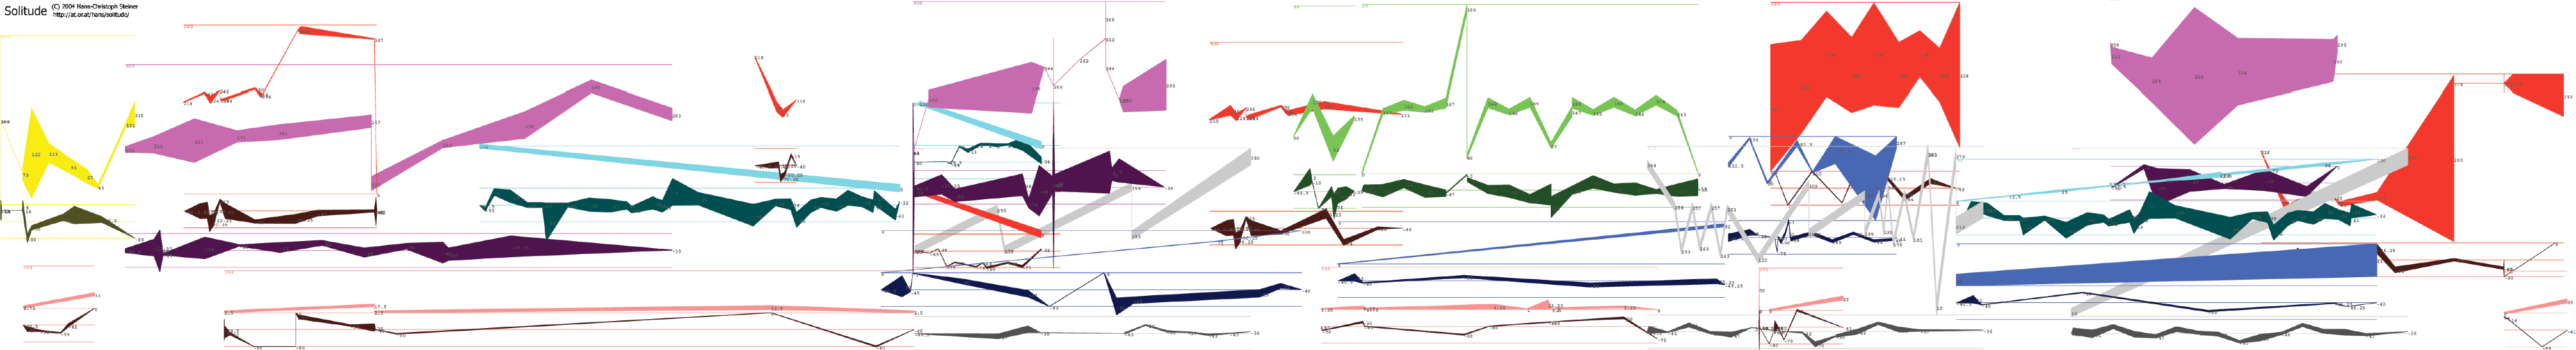
\includegraphics[width=1.0\textwidth]{img/solitude.png} 
%\captionsetup{justification=centering}
\caption{Hans-Christoph Steiner's\protect\footnotemark graphic score for Solitude, created using Pure Data's data structures. \cite{wikipedia_2020_graphic}}
\end{figure}

\todo[inline]{not sure if this score Solitude is part of CC. Might need to ask for permission.}

\footnotetext{\href{https://at.or.at/}{Hans-Christoph Steiner's site.}}

Cage, Brown and Feldman were greatly influenced by Pierre Schaeffer, a french engineer at Radiodiffusion-Television Francaise (RTF), who in 1948, presented the first musical works created with disk recorders. These were the first examples of \textit{musique concrète}\footnote{Today we would refer to it as sampled music.}, as he would call it, a style of music which is categorized by the use of recorded ordinary sounds assembled together in seemingly random ways. Schaeffer would later go on to collaborate with Pierre Henry, another notorious French composer, creating a repertoire of works for tape, including, most notably \textit{Symphonie pour un Homme Seul}, which translates to "Symphony for one man alone". (1950). The four channels were arranged in a tetrahedral configuration with two front speakers, one back speaker, and a final overhead speaker, making this one of the first examples of \textit{periphonic}\footnote{Periphonic refers to sound with height, while \textit{pantophonic} is sometimes used to denote sound systems with horizontal-only reproduction.} music. Schaeffer also helped develope the \textit{potentiomètre d'espace}, one of the first \textit{spatial audio} audio controllers which he controlled during live performances to modify the amplitude of speaker feeds. 

In Germany, another composer by the name of Karlheinz Stockhausen would soon make his own mark in the field of \textit{electro-acoustic} music. Stockhausen is perhaps the most ambitious composer of \textit{spatial music} in this era. Inspired by tape music, Stockhausen would travel to RTF, the birthplace of tape-based works, to learn about the technology. Soon after his time at RTF, he would return to Westdeutsche Rundfunk's (WDR) Studio fur Elektronische Musk\footnote{Which translates to studio for electronic music.} to create his most prolific tape pieces. \textit{Gesang der Junglinge}\footnote{Which translates to "Song of the Youths".} (1956) is considered by some as the first piece for multi-track tape. The premiere featured a number of speakers arranged \textit{panoramically} onstage \cite{zvonar1999history}. Stockhausen later remixed this piece for quadraphonic sound\footnote{Playback system which uses 4 speakers.} system. Later, in 1960, he would go on to create \textit{Kontakte}, his first truly quadraphonic piece. Stockhausen used a turntable system with a rotating speaker and four microphones to create the illusion of spinning sounds. Stockhausen also explored spatial attributes of sound in his acoustic compositions written for multiple orchestras and multiple choruses.

% the piece with the helicopters 

Then, in 1958, one of the most impactful examples of spatial electronic music would be performed. Edgar Varèse's\footnote{French-born composer (December 22, 1883 – November 6, 1965). Coined the term "sound mass" to describe his music. } \textit{Poème Électronique} was featured at the Brussels World Fair (Expo 58), a major international event with artists from all over the world. The festival attracted up to two million visitors! For the exposition of this piece, the Philips Corporation set up 15 tape recorder and over 400 loudspeakers \cite{malham19953}. This is likely one of the largest spatial music installations that have ever been accomplished. Xenakis, another giant of electro-acoustic music, designed the Philips Pavilion under the supervision of renowned Swiss-French architect Le Corbusier (1887-1965). 

\begin{figure}[ht!]%force figure here, top, strict
\centering
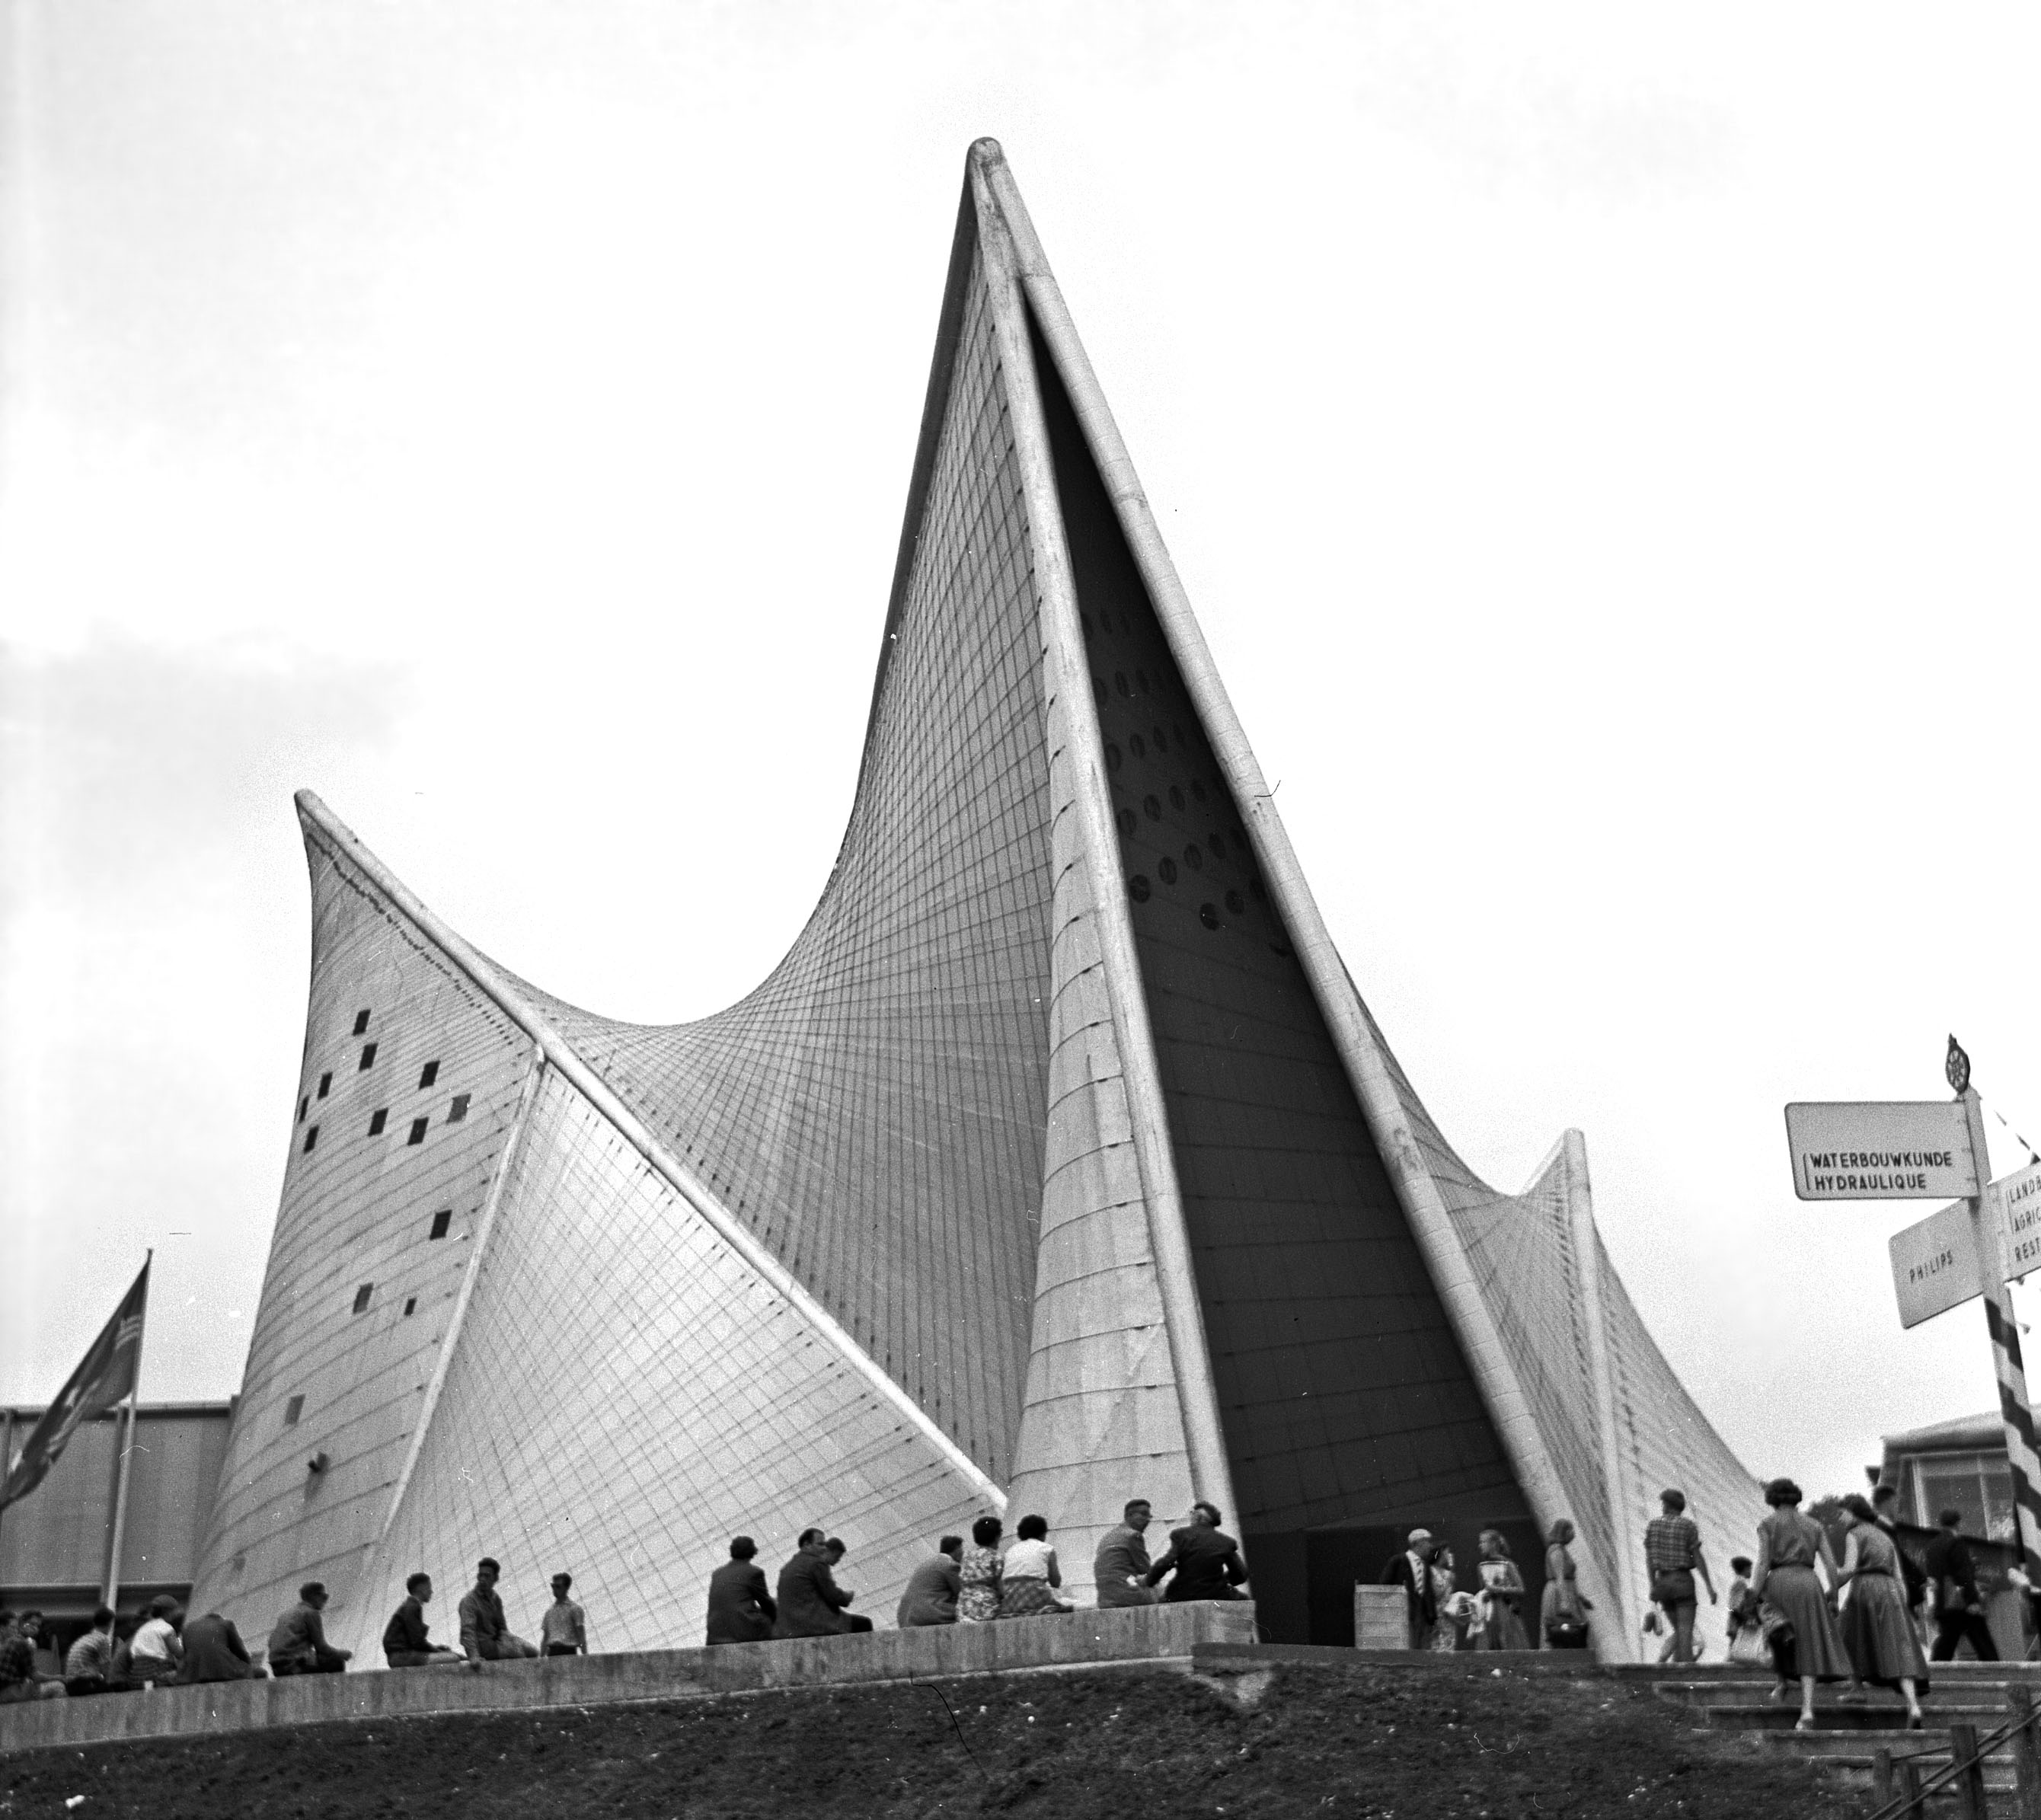
\includegraphics[width=0.6\textwidth]{img/expo58.jpg} 
%\captionsetup{justification=centering}
\caption{The Philips Pavilion \cite{wikipedia_2020_expo}}
\end{figure}

\cite{zvonar2000extremely} provides a list of the different \textit{types} of electro-acoustic works in relation to their associated techniques, along with some influential composers representative of each method:

\begin{enumerate}
    \item Live performance or "diffusion" of sound (Pierre Henry).
    \item Environmental multi-channel soundscape (John Cage).
    \item Classic studio multi-track tape composition (Karlheinz Stockhausen).
    \item Automated location control (Edgard Varèse).
\end{enumerate}

In this "live performance" setting, Pierre Henry created a repertoire of tape works which would be \textit{panned} around in real-time according to the desired trajectories manipulated by the composer. These works made use of Schaeffer's aforementioned \textit{Potentiometre d'espace} created in 1951, which translates to spatial potentiometer\footnote{A potentiometer is an electrical component which allows one to manually change the resistance between two points in a circuit.}. Examples of Cage's environmental works include \textit{HPSCHD}\footnote{Short for harpsichord.}(1960) which used 58 channels of live performers and tape. The piece was 5 hours in duration but not meant to be experienced in full, instead the audience was invited to enter and leave the space enjoying the created environment over the duration of the piece. The final two classifications refer to works which are "fixed" - suggesting that the trajectories of sounds are imprinted into the tapes and never controlled during the performance, and the works of Varèse which used an algorithm\footnote{In this case the algorithm was imprinted on tape.} to manipulate the real-time diffusion\footnote{Diffusion in this context meaning panning of sound sources in space.} of sound sources. 

John Chowning, famous for his discovery of frequency modulation (FM) as a musical technique at Stanford, also published and composed spatial pieces relevant today. \cite{chowning1971simulation} published by Chowning in 1971 is considered a seminal piece of technical literature by a pioneering computer musician detailing spatial audio. In it, Chowning describes a system for the synthesis of spatial sound relying on FM and reverb to describe moving sources. \textit{Turenas} (1972) makes use of a quadraphonic layout for this purpose and was composed at CCRMA\footnote{Center for Computer Research in Music and Acoustics at Stanford.} which he was a founding member of. It should be noted here that the substantial difference in speaker count between \textit{Poème Électronique} and \textit{Turenas} had no impact on the historical importance of these works. It is easy to believe that higher speaker count is crucial for \textit{good} spatial music works, Chowning demonstrates that it is not.

Part of the reason for the lower speaker count in some of these early works can be explained by the exorbitant cost of computers capable of handling these processes at the time. In 1981 at IRCAM\footnote{Institut de Recherche et Coordination Acoustique/Musique. Or, Institue for Research and Coordination Acoustical/Musical. It is organizationally linked to the Centre Pompidou in Paris.} the 4X synthesizer used to perform Pierre Boulez's\footnote{French composer perhaps best known for his large orchestral works featuring live electronics (26 March 1925 – 5 January 2016). Founding member of the aforementioned IRCAM.} \textit{Répons} (1985) costed \$100,000, today it is possible to recreate the synthesized elements of this piece using a personal computer. 

This brings us to the conclusion look into the history of spatial music. As we can see, while many contemporary composers might attribute the development of spatial music to composers of the 20th century, the use of spatial elements in composition has a longstanding tradition that spans hundreds of years. The next section of this text will introduce the reader to some modern composition in the field of spatial instruments music, followed by literature on capture and reproduction of spatial music, and finally a look into the use of immersive environments for spatial music in the proceeding chapters.

\section{Contemporary Spatial Music} \label{sec:contemp_works}

Several authors have explored the use of space in composition with varying degrees of success. In this section we will explore the techniques and aesthetics employed by these composers. The following pieces in this section were selected because the composers all use "spatial articulation as a central element in the musical construction\footnote{Lyon in Sound Anthology Program Notes CMJ 41:1}". Our hope is that by understanding the methods and processes used by some of these composers the reader might be better equipped to create impactful spatial music and carve their own style to differentiate themselves from the many other artists in this field. 

\subsection{Concert music}

\cite{hagan2017sound} offers an overview of some of the current leading figures in the development of spatial music. Before diving into the particular composers and their works two noteworthy facts stand out from these program notes. The first interesting information is that the delivery of the musical material\footnote{Found \href{https://muse.jhu.edu/article/656037}{here}. Jump to end of page to download audio files.} for public consumption used a stereo format with binaural properties. What this means is that the music does have spatial attributes, but much of it will be lost because the listener will not have the ability to rotate the soundfield in relation to their head orientation. The second noteworthy piece of information is that in this anthology Hagan and Lopez-Lezcano opted for \textit{static binaural synthesis} while the rest create binaural recordings - using a dummy head. This offers the listener the possibility, albeit with different materials, to experience the quality changes between both spatial audio rendering methods.

We will discuss the different pieces in order of appearance within the program notes. \textit{Spin} (2016) by Ludger Brümmer was created by taking video files and converting these into noisy sound material. The sound is then organized contrapuntally and the resulting soundfield is spun over the course of the piece. This piece was recorded at the \href{https://zkm.de/en}{ZKM Klangdom} in Germany using 32 channels. \cite{ramakrishnan2006zkm} provides a rich description of the "Kubus" which is the name of the concert hall where this piece was recorded. \textit{Spin} has a very synthetic quality to it and resembles the score someone might hear in a sci-fi film. It features noises one could qualify as other-wordly: warps, glitches and combed filters appear to be prominent. Ludger's former interests also include physical modeling and granular synthesis, both of which also appear to be exemplified here. 

\begin{figure}[ht!]%force figure here, top, strict
\centering
\includegraphics[width=0.7\textwidth]{img/zkm-commons.jpg} 
%\captionsetup{justification=centering}
\caption{ZKM - wikimedia commons}
\end{figure}

\textit{Sveti Kliment} (2007) by Robert Sazdov and was recorded at the Sonic Lab of the Sonic Arts Research Centre (SARC) in Belfast, Northern Ireland. The composition was inspired by Saint Clement of Ohrid from the Orthodox Church of Macedonia, a patron saint of education and language who committed his life to: research, teaching, and improving the lives of "those in his diocese". The piece open with the natural sound of a flute but quickly morphs into a soundscape of reversed noises and unintelligible speech snippets. The timbre of the flute reappears as a thematic motif and its reverberation is frozen and played over, using the same instrument. The timbre of the flute seems to be that of a ethnic instrument perhaps in reference to the Balkans. 

\textit{Morphons and Bions} (2011) is a real-time Puredata composition which relies on noise synthesis and randomness. \cite{hagan2012aesthetic} provides a richer description of the work. As opposed to Sazdov's piece, all the sounds in this piece are synthesized in real-time. According to Hagan: 

\begin{quote}
    "Because the work is built on a substrate entirely made of noise, the piece is situated within certain philosophical and aesthetic issues surrounding noise, its use, and its definition."
\end{quote}

Indeed, a lot of discussion has gone into the role of noise in contemporary music. Despite the abundance of noise in \textit{Morphons and Bions}, Hagan does not consider the piece to fall under the category of "noise music", given the harmonic and quasiharmonic patterns that emerge from the organization of sounds. One interesting ontological point raised by Hagan is the idea of noise being the main source of information in this work. This goes against established notions of engineers seeking to remove noise from signals. As she says: "the noise \textit{is} the signal". 

\cite{hagan2017textural} provides more technical information on the piece. Here, Hagan describes the two main synthesis method employed by this work, which were later combined into one. The first she describes as additive synthesis modulated with white noise which results in the following equation:

$$
x(t)=\sum_{k=1}^{6} w(t) \sin \left(2 \pi h(t) f_{0}(t) t+D(t) n(t)\right)
$$
where \\
$n(t)=$ white noise, \\
$D(t)=$ depth (amplitude of white noise) changing in time, \\ 
$f_{0}(t)=$ fundamental frequency changing in time, \\
$k=$ partial number, \\
$w(t)=$ Gaussian random variable with mean $1 / k$, and \\
$h(t)=$ Gaussian random variable with mean $k$.\\

As you can see the equation shows both AM and FM with noise as the modulating signal. Hagan also describes the use of band-pass filters with aleatory properties to further articulate her sounds. Hagan has adopted the terms "textural composition" to describe her music. Her work in this domain draws from the philosophical frameworks of Russolo, Cage, and Xenakis, and is driven by statistical methods, such a Gaussian distributions. \href{http://www.kerrylhagan.net/#m&b}{Her site} contains all the associated patches required to perform the piece live. Given the aleatory nature of the work, each rendition should be subtly different.

\textit{Il Prete Rosso} (2013) Charles Nichols is a work for amplified violin, motion sensor and computer, written for Sarah Plum. The piece was inspired by Antonio Vivaldi, teacher and violin virtuoso, and translates to "The Red Priest" - nickname given to Vivaldi for his red hair and ordinance. In the piece the violin is looped live and played over while recorded elements are spatialized. The computer musician interjects with a wah filter, phaser and delay effects. The motion sensor, attached to the violin player is used to control the center frequency of the wah filter. The work was premiered at the Cube of the Moss Arts Center at Virgia Tech which yields an impressive 124.4 channel system.

The fifth piece in this anthology titled \textit{He Slowly Fell, and Transformed into the Terrain} (2016) was composed by Natasha Barrett in sixth-order Ambisonics using IRCAM's Spat software. This piece is the longest from the collection lasting over 20 minutes. The composer applies HOA granular synthesis, a technique in which sounds are fragmented into thousands of smaller units for re-synthesis, applied to soundfield recordings captured using a FOA commercial microphone. An interesting aspect of the work, not mentioned in the text, is the concept of privacy. Audio recordings taken in public are problematic as source material. Certain laws exist prohibiting artists to use these materials without permission. Through the use of granular synthesis, the material quality of voices is maintained, but the dialogue because unintelligible, making this a non-issue. \cite{barrett2016musical} also references the HOA granular synthesis unit developed at IRCAM. The system, titled \textit{Grandad} encodes each individual grain of sound in 9th-order ambisonic and can be heard in the second movement of \textit{Hidden Values} (2012), also by Barrett. 

\textit{Space, S[acred|ecular]} (2015) was written by Fernando Lopez-Lezcano using impulse responses capture at Hagia Sophia: a cathedral turned mosque turned museum, featuring a reverberation time of over ten second\footnote{Depending on where the impulse response is taken.}. The building in Istanbul, Turkey, was acoustically sampled in order to recreate its sound using a new reverb technique for Higher Order Ambisonics (HOA). Fernando's use of two instruments, voice and percussion, alludes to the dual nature of the religious space.  \cite{lopez2014architecture} describes the reverb method, which consists of using an intermediary decoder for the convolution reverb. This means that the HOA reverb can be implemented even if the playback system does not support HOA. The impulse responses were processed from balloon pops using an analysis/re-synthesis method which measures echo density and energy at multiple frequency bands. The technique was informally compared in a listening test with the favoured sine swept technique to good effect \cite{abel2010estimating}. The entire piece was written in \href{https://ccrma.stanford.edu/software/snd/snd/s7.html#juce}{s7}, "a Scheme implementation [of Common Lisp Music] intended as an extension language for other applications\footnote{Scheme is a programming language which is part of the Lisp family. Lisp is one of the oldest low-level programming languages (only Fortran is older by one year).}". The mixing process, as well as the reverb, were all implemented using open source software. This included the binaural decoding which suggests that, in theory, no HDLA is needed for creating music for these systems. 

\begin{figure}[ht!]%force figure here, top, strict
\centering
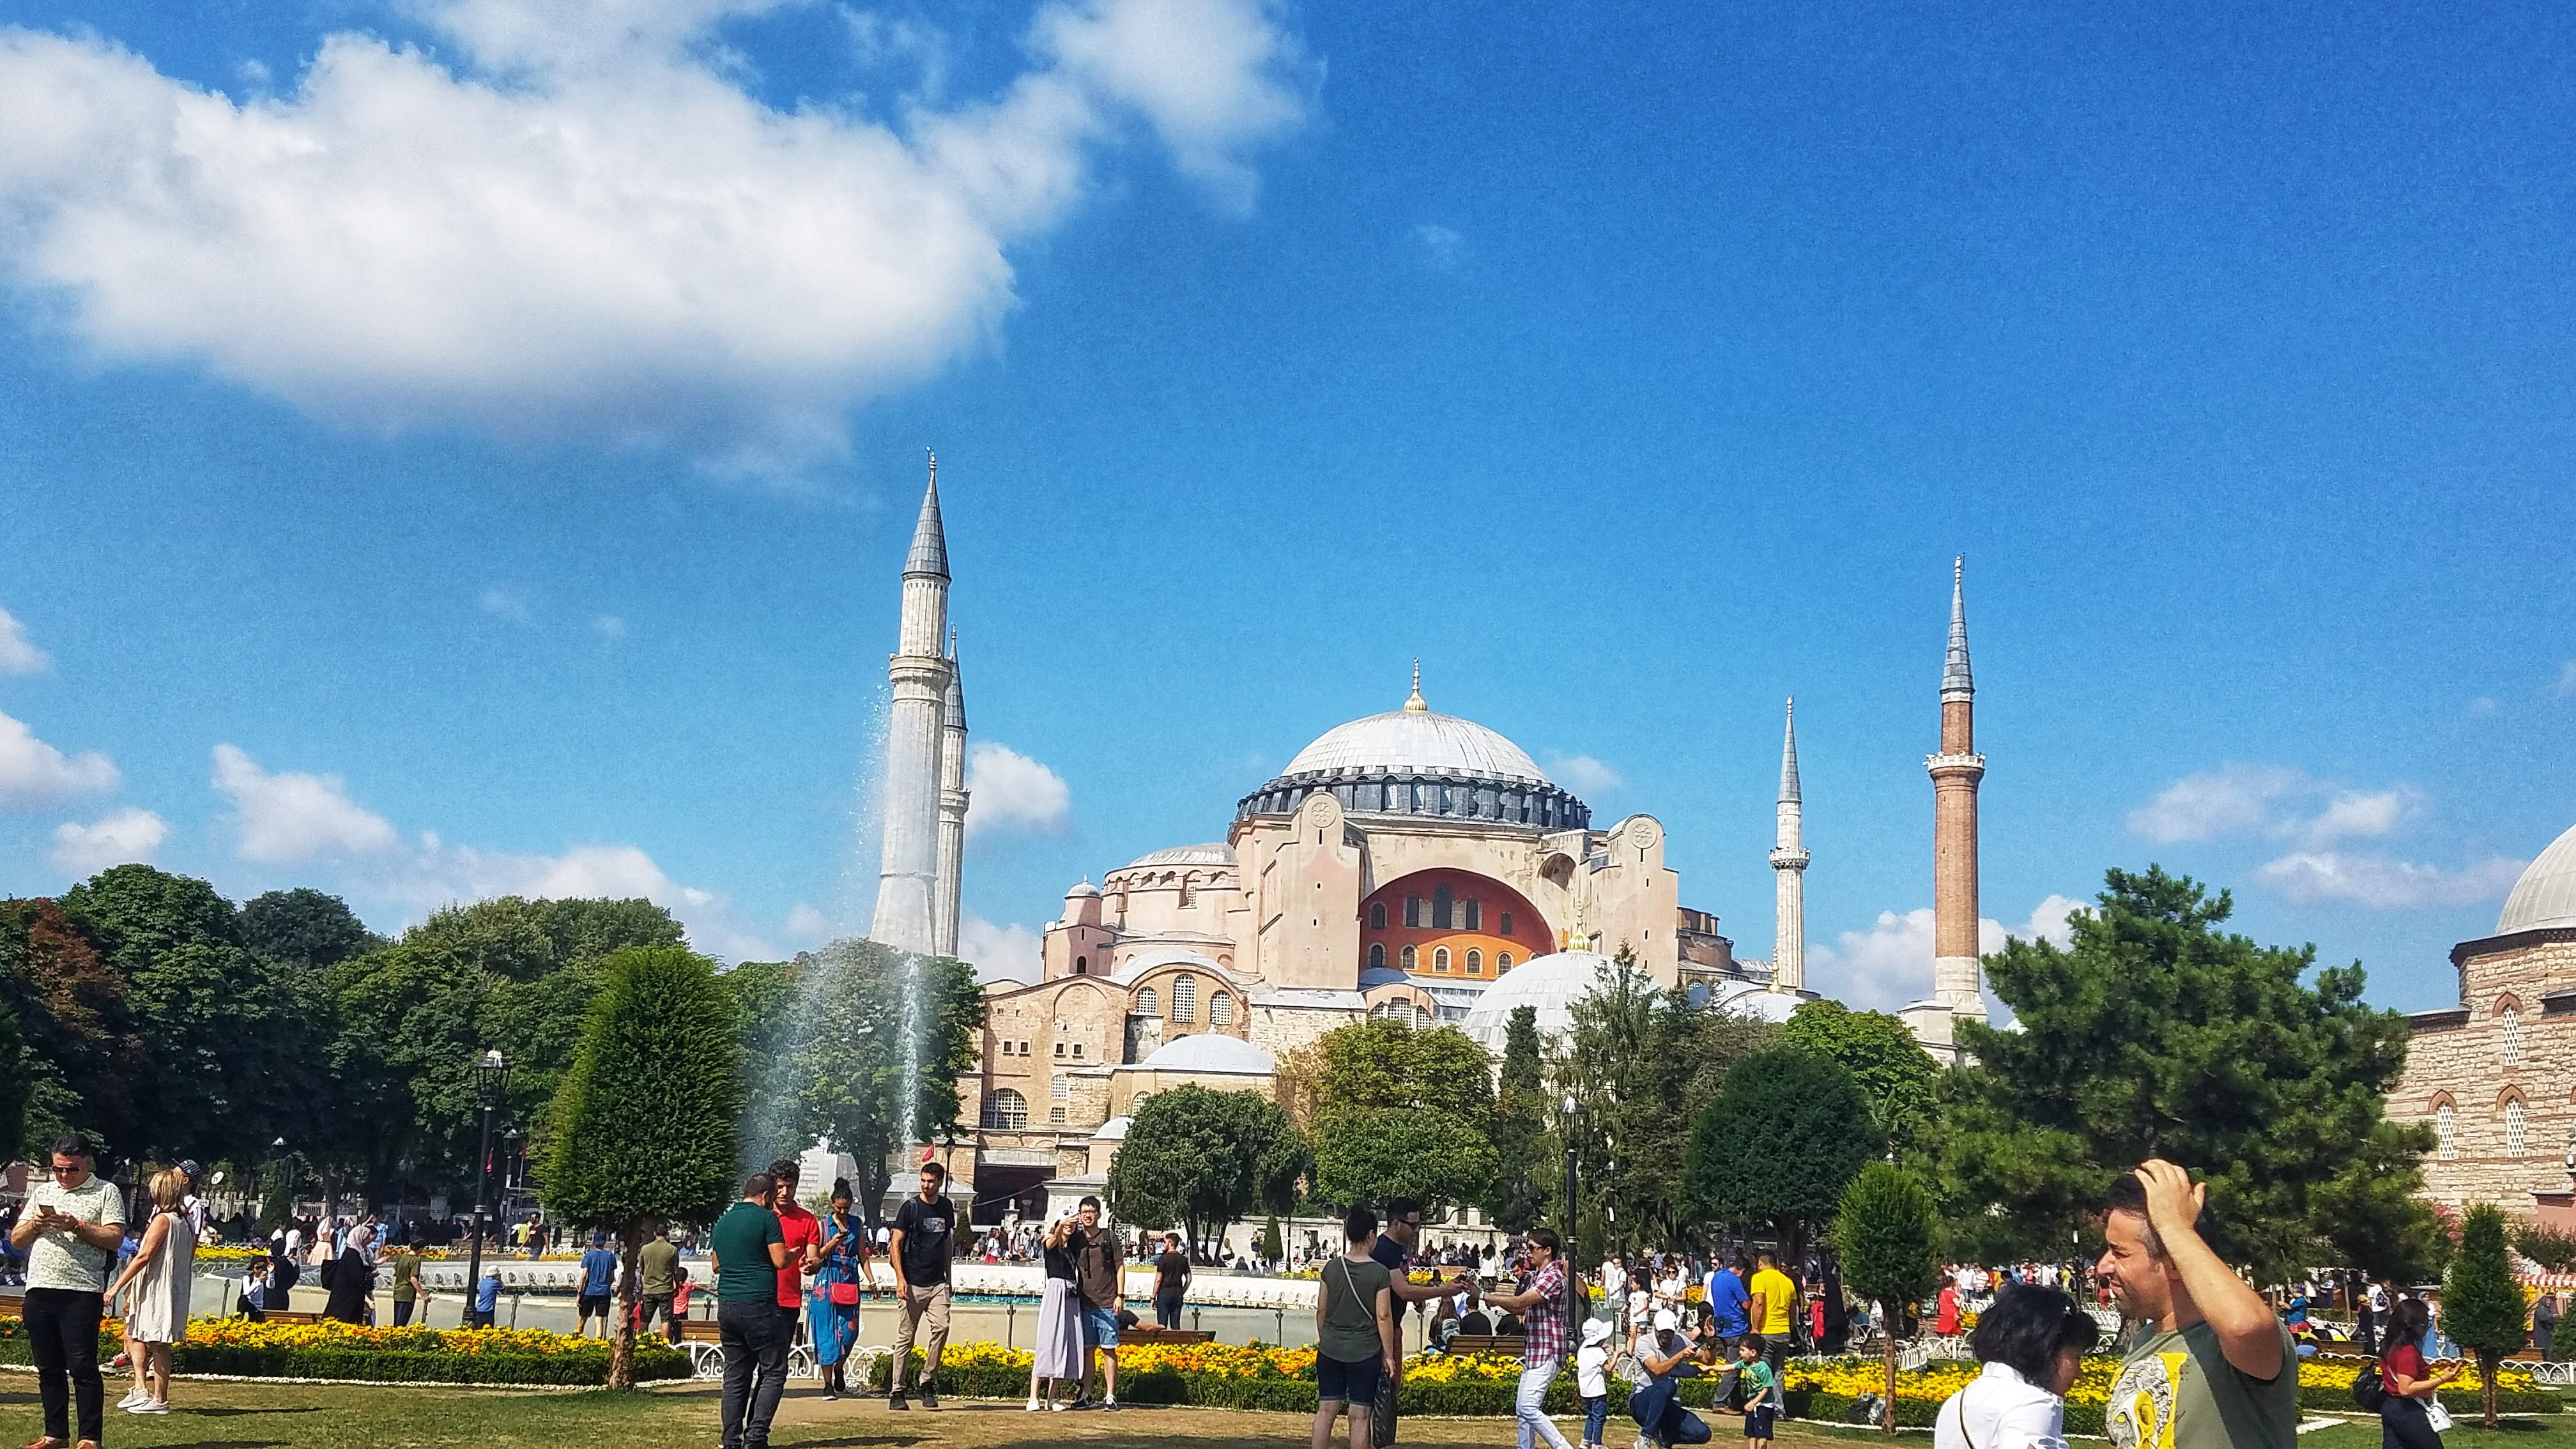
\includegraphics[width=0.7\textwidth]{img/hagia-sofia.jpg} 
%\captionsetup{justification=centering}
\caption{Hagia Sofia - wikimedia commons}
\end{figure}


The final piece discussed included in the anthology comes from Gerriet K. Sharma and is titled \textit{mirage 4} (2015). The piece was composed with and for the icosahedral\footnote{Speaker approximating a sphere with 20 faces and one speaker for each phase of the geometry.} loudspeaker developed by the Institute of Electronic Music and Acoustics (IEM) at the aforementioned ZKM\footnote{ZKM stands for "Zentrum für Kunst und Medien" which translates to "Center for Art and Media Karlsruhe", Karlsruhe the city in Germany where the cultural center is located.}. This icosahedral speaker, takes the concept of ambisonic microphones, which capture soundfields at a single point, and invert the mechanism, attempting to project a soundfield from a single point in space, with increasing resolution based on the number of transducers. 

\cite{wendt2017perception} by Wendt, Sharma, et al. discusses the ability of such a system to reproduce accurate spatial dimensions of sound for compositional means. The system is indeed capable of creating the impression of moving trajectories of sound by exploiting wall reflections which are perceived as virtual sources. These coincident speaker arrays can be considered as a portable and affordable means for spatial music reproduction. The greatest benefit these provide, for composers, is the ability to reproduce \textit{periphonic} spatial music, that is, sound with height, without having to rely on the venues' loudspeaker array. 

Ontologically, Sharma has framed his composition using the language of sculptors, discussing at length about materiality of sound, and the treatment of space as a plastic - and malleable - medium. Unfortunately, the recording included seems to suffer from significant noises, which I don't believe were intentional. These were picked up by the binaural recording system during the recording of the piece. It is however, entirely possible that these sounds \textit{are} intentional. The predominant sounds in the work are long, noisy, and soft. The piece reminds one of an ethereal, nebulous cloud, floating above them. There is a clear motif, with identical pitches reappearing at different points of the piece together with synthesized drones. 

\subsection{Installation works}
%https://escholarship.org/content/qt4d50k2fp/qt4d50k2fp.pdf

\subsection{Video games}
%  http://www.visual-memory.co.uk/b_resources/Munday%202007%20Music%20In%20Video%20Games.pdf

\subsection{XR Experiences}
% https://dl.acm.org/doi/pdf/10.1145/3359997.3365740?casa_token=En3ZeasOIT4AAAAA:pCmykPbrMvlNNHmyiiBzEhRScdcc1JyXM9R9Pl20Jsa-_rR6fMnWJIj33W0MMDZHPHrvXpR5PA

\section{Open tools for spatial music}\label{sec:open_tools_spat_mus}

This section will provide an overview of different existing tools for computer musicians which facilitate the creation of spatial music. We will focus on free and open source tools which work inn conjunction with computer music languages such as Pd, SuperCollider, Csound, etc. 

 

\section{History of Spatial Instruments} \label{sec:spat_instruments}
%older
\section{Contemporary Spatial Instruments}

This section will discuss the development of \textit{spatial instruments} in the 21st century. The term \textit{spatial instrument} refers to instruments which allow the user to manipulate spatial elements of sound. Spatial elements might include: direction, reverberance, width, etc. Traditional instruments generally allow the performer control over dynamics, pitch, and sometimes timbre. In contrast, \textit{spatial instrument} give the performer augmented control by allowing the user to modify the position of sound in space, whether that be for multi-channel sound reproduction or binaural synthesis\footnote{Virtual surround sound over headphones.}. 
Many instruments of this nature have been developed over the last few decades due to the popularity of multi-channel reproduction in electro-acoustic music. The development of such instruments goes back to the 1950s in fact, with pioneering works by composers such as Pierre Schaeffer. In contrast to our common definition of instruments, many of the interfaces which will be described in this section do not produce sound at all. In fact, much of the development in Human Computer Interaction (HCI) related to this field has focused solely on the manipulation of sound in space as separate practice from mapping controls to sound synthesis methods.  

\cite{pysiewicz2017instruments} presented a comprehensive ethnomusicological review of \textit{spatial instruments}. In that reference, the authors described a \textit{taxonomy} for the different types of spatial instruments. The three main categories from the 31 different spatialization interfaces found were: acoustic instruments extended to allow for spatial control, interfaces for the manipulation of spatial elements of sound only, and interfaces both for manipulation of spatial elements of sound as well as synthesis parameters. 

In the following sections we will describe some of the instruments created by pioneering composers from the early days of electro-acoustic music, as well as contemporary inventions which could lead to new compositional approaches. Our motivation is to understand the state-of-the-art and consider approaches which have not previously been undertaken. As we explore these different instruments we will expound upon their viability for an open-source approach to spatial music. 

\subsection{Controllers}
\subsection{Augmented instruments}
\subsection{Real-time spatial synthesis}

\section{Open Tools for Spatial Instruments}

\section{The Future of Spatial Music \& Instruments}

\section{Conclusion}



